% !TEX program = xelatex
% !TEX encoding = UTF-8

\documentclass[11pt, a4paper]{article} % use larger type; default would be 10pt

\usepackage{fontspec} % Font selection for XeLaTeX; see fontspec.pdf for documentation
\defaultfontfeatures{Mapping=tex-text} % to support TeX conventions like ``---''
\usepackage{xunicode} % Unicode support for LaTeX character names (accents, European chars, etc)
\usepackage{xltxtra} % Extra customizations for XeLaTeX
\usepackage{tikz}
\usetikzlibrary{arrows,calc,patterns}

\setmainfont[Ligatures=TeX]{[EBGaramond-Regular.ttf]} % set the main body font (\textrm), assumes Charis SIL is installed
%\setsansfont{Deja Vu Sans}
\setmonofont[Ligatures=TeX]{Fira Code}

% other LaTeX packages.....
\usepackage{fullpage}
\usepackage[top=2cm, bottom=4.5cm, left=2.5cm, right=2.5cm]{geometry}
\usepackage{amsmath,amsthm,amsfonts,amssymb,amscd,systeme}
\usepackage{unicode-math}
\usepackage{cancel}
\geometry{a4paper} 
%\usepackage[parfill]{parskip} % Activate to begin paragraphs with an empty line rather than an indent
\usepackage{fancyhdr}
\usepackage{listings}
\usepackage{graphicx}
\usepackage{hyperref}
\usepackage{multicol}

\renewcommand\lstlistingname{Algorithm}
\renewcommand\lstlistlistingname{Algorithms}
\def\lstlistingautorefname{Alg.}
\lstdefinestyle{mystyle}{
    % backgroundcolor=\color{backcolour},   
    % commentstyle=\color{codegreen},
    % keywordstyle=\color{magenta},
    % numberstyle=\tiny\color{codegray},
    % stringstyle=\color{codepurple},
    basicstyle=\ttfamily\footnotesize,
    breakatwhitespace=false,         
    breaklines=true,                 
    captionpos=b,                    
    keepspaces=true,                 
    numbers=left,                    
    numbersep=5pt,                  
    showspaces=false,                
    showstringspaces=false,
    showtabs=false,                  
    tabsize=2
}
\lstset{style=mystyle}

\newcommand\course{6 - Матстатистика}
\newcommand\hwnumber{Домашня КР №2}             % <-- homework number
\newcommand\idgroup{ФІ-91}                
\newcommand\idname{Михайло Корешков}  

\usepackage[framemethod=TikZ]{mdframed}
\mdfsetup{%
	backgroundcolor = black!5,
}
\mdfdefinestyle{ans}{%
    backgroundcolor = green!5,
    linecolor = green!50,
    linewidth = 1pt,
}

\pagestyle{fancyplain}
\headheight 35pt
\lhead{\idgroup \\ \idname}
\chead{\textbf{\Large \hwnumber}}
\rhead{\course \\ \today}
\lfoot{}
\cfoot{}
\rfoot{\small\thepage}
\headsep 1.5em

\linespread{1.2}

\begin{document}

\section*{№1}
\begin{mdframed}
    $$n = 15$$
    $$\xi_i \sim Exp(\lambda) - iid$$

    Побудувати $0.95$-довірчий інтервал для 
    \begin{itemize}
        \item $M\xi_1$
        \item $\sqrt{D\xi_1}$
    \end{itemize}
\end{mdframed}

\subsection*{1.}

Перш за все зазначу, що $M\xi_i = \frac{1}{\lambda}$.

Let $T_1(\vec X) = \overline X$. Це змістовна та незміщена оцінка $M\xi_1$.
Хочемо привести цю статистику до відомого розподілу.

Зауважу що $\chi^2(n) \sim Gamma(\frac{n}{2}, 2)$.

Спочатку перетворю $\xi_i$ наступним чином:\\
Нехай $\eta_i = 2\lambda\xi_i$.
$F_\eta(x) = F_\xi(\frac{x}{2\lambda})$.
$f_\eta(x) = \frac{\lambda}{2\lambda} e^{-\frac{\lambda}{2\lambda}x} = \frac{1}{2}e^{-\frac{x}{2}}$.
Тобто 
$$2\lambda\xi_i = \eta_i \sim \exp(\frac{1}{2}) \sim \chi^2(2)$$.

Тоді 
$$2 \lambda \sum_i \xi_i \sim \chi^2(2n)$$ 
- отримали табличний розподіл.

Let $\gamma = 0.95$.
$$P\left(g_1 < 2 \lambda \sum_i \xi_i < g_2\right) = \gamma$$
$$P\left(\frac{g_1}{2\sum_i \xi_i} <  \lambda  < \frac{g_2}{2\sum_i \xi_i}\right) = \gamma$$
$$P\left(\frac{2\sum_i \xi_i}{g_2} <  \frac{1}{\lambda}  < \frac{2\sum_i \xi_i}{g_1}\right) = \gamma$$

Використовую центральний інтервал із площею $\gamma$, залишаючи ліворуч та праворуч 
інтервали із площами $\frac{1-\gamma}{2}$ кожен. 
Це відповідає
$$g_1 = F^{-1}_{\chi^2(2n)}\left(\frac{1-\gamma}{2}\right)$$ 
$$g_2 = F^{-1}_{\chi^2(2n)}\left(\frac{1+\gamma}{2}\right)$$ 

Отримали $\gamma$-довірчий інтервал 
$$\left(\frac{2\sum_i \xi_i}{g_2} ; \frac{2\sum_i \xi_i}{g_1}\right)$$

Обчислимо його у Python:
\begin{figure}[h]
    \centering
    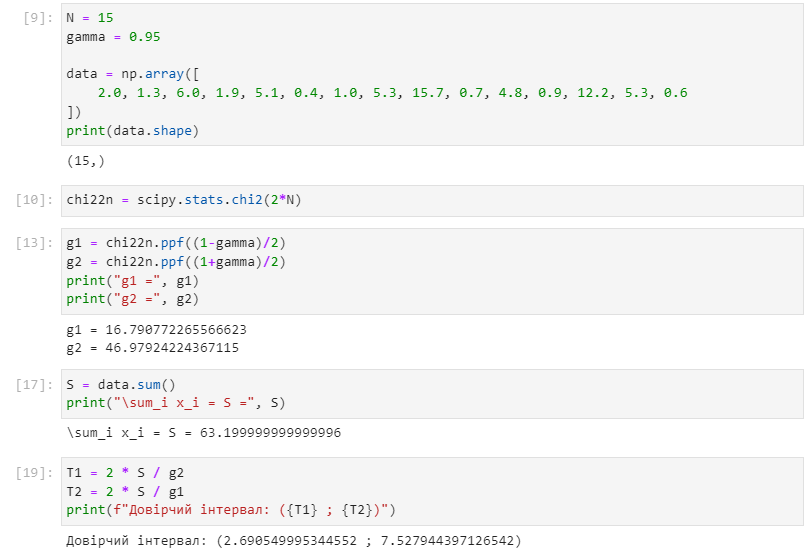
\includegraphics[width=0.9\textwidth]{img/task1.png}
\end{figure}

\begin{mdframed}[style=ans]
    Маємо $0.95$-довірчий інтервал для $M\xi_1$:
    $$P\left(2.69 < M\xi < 7.53\right) = 0.95$$
\end{mdframed}

\subsection*{2.}
Стандартне відхилення має вигляд ...

\section*{№2}



\end{document}

